% Compilation : pdflatex B1.tex (deux fois).
% Document autonome : texte, formules et figures TikZ modifiables.
% Les reperes Source renvoient aux pages du manuscrit.
\documentclass[11pt,a4paper]{article}
\usepackage[utf8]{inputenc}
\usepackage[T1]{fontenc}
\usepackage[provide=*,french]{babel}
\usepackage[scaled=.95]{helvet}
\renewcommand{\familydefault}{\sfdefault}
\usepackage{amsmath,amssymb,esint,array,tabularx}
\usepackage{geometry}
\geometry{left=15mm,right=15mm,top=18mm,bottom=18mm,headheight=14pt,headsep=6mm}
\usepackage{fancyhdr,lastpage,tikz}
\usetikzlibrary{arrows.meta,calc,decorations.pathreplacing,decorations.pathmorphing,decorations.markings,patterns}
\usepackage[most]{tcolorbox}
\usepackage{enumitem,titlesec,needspace,hyperref}
\hypersetup{hidelinks,pdftitle={Étude des sources de champ électromagnétique},pdfsubject={Cours de physique}}
\pagestyle{fancy}\fancyhf{}
\fancyhead[L]{\footnotesize Physique B1 - Étude des sources du champ électromagnétique - inspiré par les cours de Mme Mesnil}
\fancyhead[R]{\small\thepage/\pageref{LastPage}}
\fancyfoot[R]{\small PC-PC*}
\renewcommand{\headrulewidth}{0pt}
\clubpenalty=10000\widowpenalty=10000\displaywidowpenalty=10000
\setlength{\parindent}{0pt}\setlength{\parskip}{4pt}
\setlength{\abovedisplayskip}{6pt}\setlength{\belowdisplayskip}{6pt}
\AtBeginEnvironment{center}{\setlength{\topsep}{4pt}\setlength{\partopsep}{0pt}}
\setlist[itemize]{leftmargin=5mm,itemsep=3pt,topsep=3pt,label=\(\rightarrow\)}
\setlist[enumerate]{leftmargin=6mm,itemsep=3pt,topsep=3pt}
\renewcommand{\thesection}{\Roman{section}}
\renewcommand{\thesubsection}{\thesection.\arabic{subsection}}
\titleformat{\section}{\Large\bfseries}{\thesection.}{.4em}{}
\titleformat{\subsection}{\large\bfseries}{\thesubsection.}{.4em}{}[\titlerule]
\titleformat{\subsubsection}{\normalsize\bfseries}{\alph{subsubsection})}{.5em}{}
\titlespacing*{\section}{0pt}{11pt}{6pt}
\titlespacing*{\subsection}{0pt}{9pt}{5pt}
\titlespacing*{\subsubsection}{0pt}{8pt}{4pt}
\newtcolorbox{cadre}[1][]{enhanced,sharp corners,colback=white,colframe=black,boxrule=1.1pt,left=7pt,right=7pt,top=5pt,bottom=5pt,before skip=7pt,after skip=7pt,#1}
\newtcolorbox{exemple}[1][]{enhanced,breakable,sharp corners,colback=white,colframe=black,boxrule=.7pt,left=8pt,right=8pt,top=6pt,bottom=6pt,before skip=8pt,after skip=8pt,#1}
\tcbset{etoiles/.style={width=\dimexpr\linewidth-22mm\relax,overlay={\node[anchor=west,inner sep=0pt,font=\small] at ([xshift=2mm]frame.east) {\(#1\)};}}}
\newcommand{\zone}[1]{\tikz[baseline=(z.base)]\node[draw,circle,inner sep=1pt,font=\scriptsize,minimum size=3.5mm](z){#1};}
\newcommand{\dd}{\mathrm d}
\newcommand{\vv}{\vec v}
\newcommand{\grad}{\overrightarrow{\mathrm{grad}}}
\newcommand{\pd}[2]{\frac{\partial #1}{\partial #2}}
\newcommand{\ux}{\vec u_x}\newcommand{\uy}{\vec u_y}\newcommand{\uz}{\vec u_z}
\newcommand{\cste}{\mathrm{cste}}
\newcommand{\titr}[1]{\par\Needspace{4\baselineskip}\textbf{\underline{#1}}\par\nopagebreak[3]}
\newcommand{\planpart}[2]{\par\vspace{5pt}{\bfseries #1. #2}\par}
\newcommand{\plansub}[2]{\hspace*{7mm}{\itshape #1) #2}\par}
\newcommand{\plansubsub}[1]{\hspace*{15mm}{\itshape #1}\par}
\tikzset{>=Stealth,every node/.style={font=\small},flow/.style={thick,->},edge/.style={thick}}
\newcommand{\etoiles}[1]{\foreach \i in {1,...,#1}{\mathord{\star}\,}}
% Figures vectorielles : toutes les coordonnées et toutes les étiquettes sont modifiables.
\definecolor{charge}{RGB}{155,50,165}
\definecolor{current}{RGB}{195,40,45}
\tikzset{chg/.style={draw=charge,thick},cur/.style={current,thick,->},plane/.style={blue!55!black,thin},pt/.style={circle,fill,inner sep=1.2pt},arr/.style={thick,->}}
\newcommand{\vj}{\vec j}
\newcommand{\sym}{\operatorname{sym}}
\newcommand{\fig}[1]{\begin{center}#1\end{center}}
\newcommand{\blob}{\draw[chg,fill=charge!8](-1.3,-.8)..controls(-1.9,.1)and(-1.1,.4)..(-.9,.8)..controls(-.7,1.3)and(-.2,.6)..(.3,1)..controls(1.7,1.4)and(1.6,.2)..(1.1,-.6)..controls(.8,-1.2)and(-.7,-1.2)..cycle;}
\newcommand{\volumefig}[1]{\begin{tikzpicture}[scale=.65]\blob\node[pt]at(0,0){};\node[above right]at(0,0){$#1$};\end{tikzpicture}}
\newcommand{\slabfig}{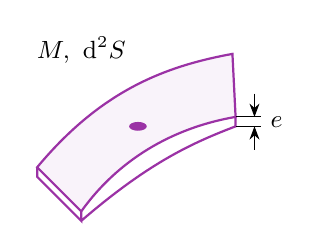
\begin{tikzpicture}[scale=.8]
\draw[chg,fill=charge!6](0,0)..controls(1,1.2)and(2,1.6)..(3.1,1.8)--(3.15,.8)..controls(2,.6)and(1.2,0)..(.7,-.7)--cycle;
\draw[chg](0,0)--(0,-.15)--(.7,-.85)--(.7,-.7)(.7,-.85)..controls(1.8,.1)and(2.5,.4)..(3.15,.65)--(3.15,.8);
\fill[charge](1.6,.65)ellipse(.14 and .07);\node[above]at(.7,1.5){$M,\ \dd^2S$};
\draw[thin](3.15,.65)--(3.55,.65)(3.15,.8)--(3.55,.8);\draw[->](3.45,.28)--(3.45,.65);\draw[->](3.45,1.17)--(3.45,.8);\node[right]at(3.55,.72){$e$};\end{tikzpicture}}
\newcommand{\wirefig}{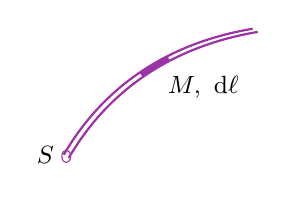
\begin{tikzpicture}[scale=.8]
\draw[chg](0,0)..controls(.7,1.2)and(1.8,1.8)..(3,2);\draw[chg](.08,-.05)..controls(.78,1.15)and(1.88,1.75)..(3.08,1.95);
\draw[charge](.04,-.025)ellipse(.07 and .1);\node[left]at(0,0){$S$};
\draw[charge,line width=2pt] plot[domain=.46:.60,samples=20] ({.04+2.1*\x+1.2*\x^2-.3*\x^3},{-.025+3.6*\x-1.8*\x^2+.2*\x^3});\node[below right]at(1.5,1.4){$M,\ \dd\ell$};\end{tikzpicture}}
% #1 : 0 symétrie des charges ; 1 antisymétrie ; 2 symétrie des courants ; 3 antisymétrie des courants.
\newcommand{\symfig}[1]{\begin{tikzpicture}[scale=.75]
\draw[fill=charge!9,chg](-1.7,0)..controls(-1.9,1.4)and(-.4,1.7)..(0,.9)..controls(.4,1.7)and(1.9,1.4)..(1.7,0)..controls(1.7,-1.6)and(.5,-1.6)..(0,-.9)..controls(-.5,-1.6)and(-1.7,-1.6)..cycle;
\ifnum#1=1\fill[green!22](0,.9)..controls(.4,1.7)and(1.9,1.4)..(1.7,0)..controls(1.7,-1.6)and(.5,-1.6)..(0,-.9)--cycle;\fi\draw[plane](0,-1.8)--(0,1.8)--(.65,2.2);\node[blue!55!black,below]at(0,-1.8){$\Pi$};
\draw[dashed](-.9,0)--(.9,0);\node[pt]at(-.9,0){};\node[pt]at(.9,0){};\node[below left]at(-.9,0){$P$};\node[below right]at(.9,0){$P'$};
\ifnum#1<2\node[charge]at(-.85,.65){$\rho$};\ifnum#1=1\node[green!45!black]at(.85,.65){$-\rho$};\else\node[charge]at(.85,.65){$\rho$};\fi
\else\draw[cur](-.9,0)--(-1.4,.8)node[above left]{$\vj(P,t)$};
\ifnum#1=2\draw[cur](.9,0)--(1.4,.8)node[above right]{$\vj(P',t)$};
\else\draw[green!45!black,->,thick](.9,0)--(1.4,.8)node[above right,align=center]{$\sym_\Pi[\vj(P,t)]$};\draw[cur](.9,0)--(.4,-.8);\node[current,right]at(.65,-1.55){$\vj(P',t)$};\fi\fi
\end{tikzpicture}}
\newcommand{\pairfig}[1]{\begin{tikzpicture}[scale=.8]\draw[plane](0,-1.1)--(0,1.2)node[above]{$\Pi$};\node[pt,charge]at(-1,0){};\node[pt,charge]at(1,0){};\node[below,charge]at(-1,0){$q$};\node[below,charge]at(1,0){$#1 q$};\end{tikzpicture}}
\newcommand{\ballplanes}[1]{\begin{tikzpicture}[scale=.8]
\ifnum#1=1\fill[charge!25](0,1)arc(90:270:1)--cycle;\fill[green!25](0,-1)arc(-90:90:1)--cycle;\else\fill[charge!15](0,0)circle(1);\fi
\draw[chg](0,0)circle(1);\draw[plane](0,-1.5)--(0,1.5)--(.6,1.8)node[right]{$\Pi_2$};
\ifnum#1=0\draw[plane](-1.6,.35)--(1.6,-.4)node[right]{$\Pi_1$};\node[charge,right]at(1.1,.8){$\rho=\cste$};\else\node[charge,left]at(-1,.7){$+\rho$};\node[green!45!black,right]at(1,.7){$-\rho$};\fi\end{tikzpicture}}
\newcommand{\ring}[1]{\begin{tikzpicture}[scale=.8]\draw[chg](0,0)ellipse(1.2 and .45);\draw[->](0,-1.3)--(0,1.7)node[above]{$\Delta$};\node[right]at(1.3,.3){$#1$};\end{tikzpicture}}
\newcommand{\cylinder}[1]{\begin{tikzpicture}[scale=.75]
\draw[chg](-1,0)ellipse(1 and .35);\draw[chg](-2,0)--(-2,2.1)(0,0)--(0,2.1);\draw[chg](-1,2.1)ellipse(1 and .35);
\draw[dashed](-1,-.6)--(-1,2.6);\draw[->](-1,2.6)--(-1,3)node[above]{$\Delta$};\node[right]at(.2,1.4){$\rho=\cste$};
\ifnum#1=1\draw[dashed](-1,1.15)--(-1.65,.8)(-1,1.15)--(-.35,.8);\node[below]at(-1.65,.8){$P$};\node[below]at(-.35,.8){$P'$};\fi\end{tikzpicture}}
\newcommand{\infcylinder}{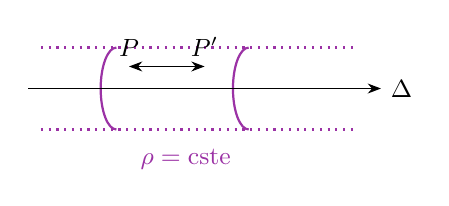
\begin{tikzpicture}[scale=.8]\draw[chg,dotted](-2,.65)--(3,.65)(-2,-.65)--(3,-.65);\draw[chg](-.8,.65)arc(90:270:.25 and .65)(1.3,.65)arc(90:270:.25 and .65);\draw[->](-2.2,0)--(3.4,0)node[right]{$\Delta$};\node[charge,below]at(.3,-.8){$\rho=\cste$};\draw[<->](-.6,.35)--(.6,.35);\node[above]at(-.6,.35){$P$};\node[above]at(.6,.35){$P'$};\end{tikzpicture}}
\newcommand{\sheet}[1]{\begin{tikzpicture}[scale=.8]
\ifnum#1=0
\draw[plane](-2,-.9)--(1.8,-.9)--(2.6,1.1)--(-1.2,1.1)--cycle;
\draw[->](.2,0)--(1.6,.8)node[right]{$\Delta_1$};\draw[->](.2,0)--(.95,-.4)node[right]{$\Delta_2$};\node[charge]at(-.9,-.35){$\sigma=\cste$};
\else
\draw[plane](-2.3,-1.15)--(2.1,-1.15)--(3,1.4)--(-1.4,1.4)--cycle;
\draw[->](.55,.05)--(1.7,.8)node[right]{$\Delta_1$};
\draw[->](.55,.05)--(1.1,-.55)node[right]{$\Delta_2$};
\draw[cur](-1.35,-.45)--(-.6,.25);\node[current]at(-.6,.77){$\vj_s=\vec{\cste}$};
\fi\end{tikzpicture}}
% #1 : 0 cylindre de courant ; 1 plan transverse ; 2 prolongement infini.
\newcommand{\solenoid}[1]{\begin{tikzpicture}[scale=.8]
\draw[thick](-1,-.7)--(2,-.7)(-1,.7)--(2,.7);
\ifnum#1=2
\draw[dashed](-1,0)ellipse(.3 and .7)(2,0)ellipse(.3 and .7);
\draw[dashed](-2,-.7)--(-1,-.7)(2,-.7)--(3.2,-.7)(-2,.7)--(-1,.7)(2,.7)--(3.2,.7);
\else\draw[thick](-1,0)ellipse(.3 and .7)(2,0)ellipse(.3 and .7);\fi
\foreach\x in{-.55,0,.55,1.1,1.65}{\draw[current,thick,postaction={decorate},decoration={markings,mark=at position .5 with {\arrow{Stealth}}}](\x,.7)arc[start angle=90,end angle=270,x radius=.3,y radius=.7];}
\draw[dotted,->](2,0)--(3,0)node[right]{$\Delta$};
\ifnum#1=1\draw[plane](0,-1.1)--(0,1.1)--(.5,1.4);\node[blue!55!black,below]at(0,-1.1){$\Pi$};\fi\end{tikzpicture}}
\newcommand{\currentring}[1]{\begin{tikzpicture}[scale=.85]
\draw[current,thick](0,0)ellipse(1.15 and .5);\draw[cur](.1,-.5)--(.4,-.47);\draw[cur](-.1,.5)--(-.4,.47);
\ifnum#1=0\draw[plane](-1.8,-.9)--(1.6,-.9)--(2.1,1)--(-1.3,1)--cycle;\node[blue!55!black,below]at(-1.8,-.9){$\Pi$};\else\draw[dashed](0,-1.1)--(0,0);\draw[->](0,0)--(0,1.5)node[above]{$\Delta$};\fi\end{tikzpicture}}
\begin{document}
{\raggedright\fontsize{27}{31}\selectfont\bfseries Étude des sources de champ électromagnétique\par}
\vspace{4mm}
\begingroup\setlength{\parskip}{.7pt}
\planpart{I}{Introduction}
\planpart{II}{Distribution de charges}
\plansub{1}{Densité volumique de charges}
\plansub{2}{Cas limite d'une distribution surfacique}
\plansub{3}{Cas limite d'une distribution linéique}
\plansub{4}{Propriétés de symétrie}
\plansubsub{a) Symétrie plane}\plansubsub{b) Antisymétrie plane}\plansubsub{c) Invariance par translation}\plansubsub{d) Invariance par rotation}\plansubsub{e) Distributions de haute symétrie}
\planpart{III}{Distribution de courants}
\plansub{1}{Vecteur densité de courant}\plansub{2}{Intensité du courant traversant une surface}\plansub{3}{Quelques ordres de grandeur pour le cuivre}\plansub{4}{Cas limite d'une distribution surfacique}\plansub{5}{Cas limite d'une distribution linéique}\plansub{6}{Propriétés de symétrie}
\plansubsub{a) Symétrie plane}\plansubsub{b) Antisymétrie plane}\plansubsub{c) Invariance par translation}\plansubsub{d) Invariance par rotation}\plansubsub{e) Distributions de haute symétrie}
\par\vspace{4pt}\textbf{Tableau récapitulatif}\par\endgroup
% Source 1
\medskip
\begingroup\setlist[itemize]{itemsep=0pt,topsep=2pt}
L'électromagnétisme est né au XVIII\textsuperscript{e} siècle.
\begin{itemize}\item Benjamin Franklin.\item Cavendish.\item Coulomb.\end{itemize}
\titr{Première moitié du XIX\textsuperscript{e} siècle}
\begin{itemize}\item Volta : invention de la pile.\item Oersted : création d'un champ $\vec B$ avec un courant.\item Ohm.\item Gauss.\end{itemize}
\titr{1831--1835 : induction}
\begin{itemize}\item Faraday.\item Lenz.\item Henry.\end{itemize}
% Source 2
\titr{Deuxième moitié du XIX\textsuperscript{e} siècle}
\begin{itemize}\item Foucault.\item Maxwell : équations de Maxwell.\item Hall : effet de Hall.\item Tesla.\item Hertz.\item Thomson.\item Lorentz.\end{itemize}
\titr{Fin du XIX\textsuperscript{e} siècle : applications de l'électromagnétisme}
\begin{itemize}\item 1870 : dynamo.\item 1875 : téléphone.\item 1878 : ampoule électrique.\item 1883 : alternateur.\item 1887 : moteur électrique.\item 1910 : tube néon.\item 1910 : oscilloscope.\item 1900 : radio.\item 1939 : magnétophone.\item 1970 : calculatrices de poche.\item 1980 : ordinateurs.\item Années 2000 : Wi-Fi, fours à micro-ondes, etc.\end{itemize}
% Source 3
\titr{XX\textsuperscript{e} siècle}
\begin{itemize}\item Physique relativiste.\item Physique quantique.\end{itemize}
\endgroup
\section{Introduction}
\textbf{Buts du chapitre :}
\begin{itemize}\item Modéliser des distributions de charges et de courants.\item Étudier l'origine de la création d'un champ électromagnétique.\end{itemize}
Dans ce cours, on se place :
\begin{itemize}\item dans le cadre de l'approximation des milieux continus ;\item à l'échelle mésoscopique.\end{itemize}
\clearpage
\section{Distribution de charges}
\subsection{Densité volumique de charges}
% Source 4 : photographie intégralement retranscrite.
À l'échelle mésoscopique, le caractère discontinu de la matière et de l'électricité disparaît. La distribution des charges est en apparence continue.
\fig{\volumefig{M}}
Considérons un « petit » volume mésoscopique $\dd^3\tau$ autour d'un point $M$. Soit $\dd^3q$ la charge qu'il contient.
\begin{cadre}La \textbf{densité volumique} $\rho(M,t)$ de charges au point $M$ à l'instant $t$ est définie par :
\[\rho(M,t)=\frac{\dd^3q}{\dd^3\tau}.\]\end{cadre}
Elle se mesure en $\mathrm{C\,m^{-3}}$. C'est l'analogue d'une masse volumique (distribution de masse).
On écrit encore que la charge élémentaire $\dd^3q$ contenue dans le volume élémentaire $\dd^3\tau$ est :
\begin{cadre}\[\dd^3q=\rho(M,t)\dd^3\tau.\]\end{cadre}
\begin{exemple}\textbf{Exemple}\par
On assimile le noyau de l'atome d'hydrogène à une sphère de rayon $R=1\ \text{fermi}=1\cdot10^{-15}\,\mathrm m$ portant la charge totale $q=e$ uniformément répartie.
La densité volumique de charge du noyau de l'atome d'hydrogène est donc :
\[\rho=\frac{e}{\frac43\pi R^3}=4\cdot10^{25}\,\mathrm{C\,m^{-3}}.\]\end{exemple}
Si la densité volumique de charges n'est pas uniforme, il faut bien prendre garde à intégrer cette densité de charges sur le volume considéré.
\begin{center}\begin{minipage}{.25\linewidth}\centering\volumefig{V}\end{minipage}\begin{minipage}{.7\linewidth}
\[\underbrace{q(t)}_{\substack{\text{charge contenue}\\\text{dans }V}}=\iiint_V\underbrace{\rho(M,t)}_{\text{intégration de }\rho(M,t)}\dd^3\tau.\]
\end{minipage}\end{center}
\subsection{Cas limite d'une distribution surfacique}
% Source 5
\fig{\slabfig}
Il arrive souvent qu'une distribution de charges soit répartie dans un volume dont l'une des dimensions, $e$, est très petite devant les autres. Tant que l'on cherche à calculer le champ assez loin de cette zone (à des distances grandes devant $e$), elle pourra être assimilée à une surface chargée.
\begin{cadre}On définit la \textbf{densité surfacique de charge} $\sigma(M,t)$ au voisinage d'un point $M$ à l'instant $t$ :
\[\sigma(M,t)=\frac{\dd^2q}{\dd^2S}.\]\end{cadre}
$\dd^2q$ est la charge contenue dans le volume élémentaire de base $\dd^2S$ et d'épaisseur $e$ entourant le point $M$.
La densité surfacique de charge $\sigma(M,t)$ se mesure en $\mathrm{C\,m^{-2}}$.
On écrit encore que la charge élémentaire $\dd^2q$ contenue dans la surface élémentaire $\dd^2S$ est donnée par :
\begin{cadre}\[\dd^2q=\sigma(M,t)\dd^2S.\]\end{cadre}
\begin{exemple}\textbf{Exemples pratiques :}
\begin{itemize}\item Tout conducteur parfait a des charges en surface.\item Un condensateur plan.\item Un ballon de baudruche frotté.\item Une bulle de savon.\end{itemize}\end{exemple}
\subsection{Cas limite d'une distribution linéique}
% Source 6
\fig{\wirefig}
De même, on rencontrera des distributions de charges réparties dans des volumes dont deux des dimensions sont très petites devant la troisième. Tant que l'on ne cherche pas à calculer le champ trop près de cette zone, elle pourra être assimilée à une distribution linéique chargée.
\begin{cadre}On définit alors la \textbf{densité linéique de charge} $\lambda(M,t)$ au voisinage d'un point $M$ à l'instant $t$ :
\[\lambda(M,t)=\frac{\dd q}{\dd\ell}.\]\end{cadre}
$\dd q$ est la charge contenue dans le volume élémentaire de longueur $\dd\ell$ entourant le point $M$.
La charge linéique $\lambda(M,t)$ se mesure en $\mathrm{C\,m^{-1}}$.
On écrit encore que la charge portée par une longueur élémentaire $\dd\ell$ est :
\begin{cadre}\[\dd q=\lambda(M,t)\dd\ell.\]\end{cadre}
\begin{exemple}\textbf{Exemples :} les antennes émettrices et réceptrices, ainsi que les cheveux.\end{exemple}
\begin{center}
\begin{minipage}{.31\linewidth}\centering\volumefig{\dd^3\tau}\[\dd^3q=\rho(M,t)\dd^3\tau\]\end{minipage}\hfill
\begin{minipage}{.32\linewidth}\centering\slabfig\[\dd^2q=\sigma(M,t)\dd^2S\]\end{minipage}\hfill
\begin{minipage}{.32\linewidth}\centering\wirefig\[\dd q=\lambda(M,t)\dd\ell\]\end{minipage}
\end{center}
% Source 7
\[\sigma(M,t)=\lim_{e\to0}\rho(M,t)e,\qquad\lambda(M,t)=\lim_{S\to0}\rho(M,t)S.\]
\subsection{Propriétés de symétrie}
\subsubsection{Symétrie plane}
\begin{center}\begin{minipage}{.43\linewidth}\centering\symfig{0}\end{minipage}\begin{minipage}{.53\linewidth}
Si $P\in\mathcal D$, alors $P'=\sym_\Pi(P)\in\mathcal D$ : c'est la condition géométrique.
\[\rho(P,t)=\rho(P',t).\]
C'est la condition sur la charge.
\end{minipage}\end{center}
\begin{cadre}Une distribution de charges est \textbf{invariante par symétrie par rapport au plan $(\Pi)$} si, pour tout point $P$ de la distribution, son symétrique $P'$ par rapport au plan $(\Pi)$ appartient à la distribution et porte la même charge que $P$ : $\rho(P,t)=\rho(P',t)$.
$(\Pi)$ est un plan de symétrie de la distribution de charges.\end{cadre}
% Source 8
\begin{exemple}\textbf{Exemples :}
\begin{center}\ballplanes{0}\hspace{7mm}\pairfig{}\hspace{7mm}
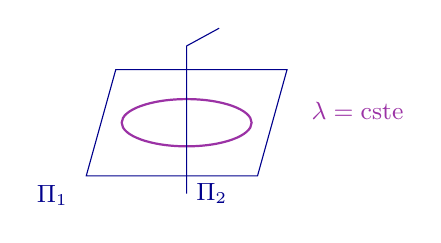
\begin{tikzpicture}[scale=.75]\draw[chg](0,0)ellipse(1.1 and .4);\draw[plane](-1.7,-.9)--(1.2,-.9)--(1.7,.9)--(-1.2,.9)--cycle;\node[blue!55!black,below left]at(-1.85,-.9){$\Pi_1$};\draw[plane](0,-1.2)--(0,1.3)--(.55,1.6);\node[blue!55!black,right]at(0,-1.2){$\Pi_2$};\node[charge,right]at(1.95,.2){$\lambda=\cste$};\end{tikzpicture}\end{center}\end{exemple}
\subsubsection{Antisymétrie plane}
\begin{center}\begin{minipage}{.43\linewidth}\centering\symfig{1}\end{minipage}\begin{minipage}{.53\linewidth}
Si $P\in\mathcal D$, alors $P'=\sym_\Pi(P)\in\mathcal D$.
\[\rho(P,t)=-\rho(P',t).\]\end{minipage}\end{center}
% Source 9
\begin{cadre}Une distribution de charges \textbf{possède un plan d'antisymétrie $(\Pi)$} si, pour tout point $P$ de la distribution, son symétrique $P'$ par rapport au plan $(\Pi)$ appartient à la distribution et porte une charge opposée à celle de $P$ : $\rho(P',t)=-\rho(P,t)$.\end{cadre}
\begin{exemple}\textbf{Exemples :}\fig{\ballplanes{1}\hspace{22mm}\pairfig{-}}\end{exemple}
\textbf{Remarque :} sur un plan d'antisymétrie, la charge est nulle.
\subsubsection{Invariance par translation}
\begin{cadre}Une distribution de charges est \textbf{invariante par translation parallèle à une direction $(D)$} si, pour tout point $P$ de la distribution, ses translatés parallèlement à $(D)$ appartiennent à la distribution et portent la même charge que $P$.\end{cadre}
\begin{exemple}\textbf{Exemples :}
\begin{itemize}\item Un cylindre infini, chargé uniformément.\end{itemize}
\fig{\infcylinder}
La distribution est invariante par translation parallèle à $\Delta$.
% Source 10
\begin{itemize}\item Un fil infini chargé uniformément.\end{itemize}
\fig{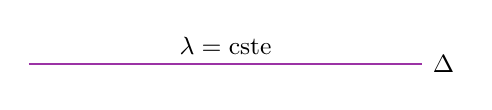
\begin{tikzpicture}\draw[chg](-2.5,0)--(2.5,0)node[right]{$\Delta$};\node[above]at(0,0){$\lambda=\cste$};\end{tikzpicture}}
\begin{itemize}\item Un plan infini uniformément chargé.\end{itemize}
\fig{\sheet{0}}
La distribution est invariante par translation parallèle à $\Delta_1$, parallèle à $\Delta_2$ et parallèle à tout axe contenu dans le plan.
\end{exemple}
% Source 11
\textbf{Remarques :}
\begin{itemize}\item Tout plan perpendiculaire à $(D)$ est un plan de symétrie.\item L'invariance par translation suppose une extension infinie de la distribution de charges. En pratique, cela signifie qu'une dimension de la distribution est très grande devant les autres longueurs de la distribution.\end{itemize}
\subsubsection{Invariance par rotation}
\begin{cadre}Une distribution de charges est \textbf{invariante par rotation autour de l'axe $(\Delta)$} si, pour tout point $P$ de la distribution, ses transformés par les rotations d'axe $(\Delta)$ appartiennent à la distribution et portent la même charge que $P$.
$(\Delta)$ est un axe de révolution ; la distribution possède la symétrie de révolution d'axe $(\Delta)$.\end{cadre}
\begin{exemple}\textbf{Exemples :}
\begin{center}\cylinder{1}\hspace{8mm}\ring{\lambda=\cste}\hspace{8mm}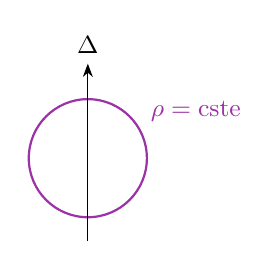
\begin{tikzpicture}[scale=.75]\draw[chg](0,0)circle(1);\draw[->](0,-1.4)--(0,1.6)node[above]{$\Delta$};\node[charge,right]at(.9,.8){$\rho=\cste$};\end{tikzpicture}\end{center}
Les distributions sont invariantes par rotation d'axe $\Delta$. Le schéma central représente un anneau chargé.
\end{exemple}
% Source 12
\textbf{Remarque :} tout plan contenant un axe de révolution est un plan de symétrie.
\subsubsection{Distributions de haute symétrie}
Si la distribution de charges possède un grand nombre de propriétés de symétrie, elle est dite de haute symétrie et sa description se simplifie.
\begin{cadre}Une distribution de charges possède la \textbf{symétrie cylindrique} si elle est invariante par rotation autour d'un axe et par translation parallèlement à cet axe.\end{cadre}
\fig{\infcylinder}
La distribution possède la symétrie cylindrique par rapport à $\Delta$.
% Source 13
\begin{cadre}Une distribution de charges possède la \textbf{symétrie sphérique} si elle est invariante par rotation autour de tout axe passant par un même point $O$. La densité de charges ne dépend alors que de la distance à $O$.\end{cadre}
\fig{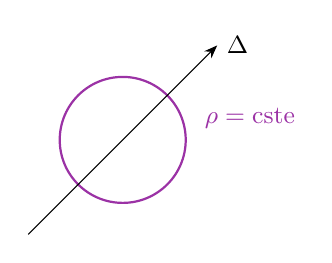
\begin{tikzpicture}[scale=.8]\draw[chg](0,0)circle(1);\draw[->](-1.5,-1.5)--(1.5,1.5)node[right]{$\Delta$};\node[charge,right]at(1.15,.35){$\rho=\cste$};\end{tikzpicture}}
\section{Distribution de courants}
Le courant électrique correspond à un transport de charges électriques résultant d'un mouvement d'ensemble de particules chargées.
Dans un conducteur métallique, les porteurs de charges sont les électrons de conduction.
Dans un électrolyte, les porteurs de charges sont les anions et les cations.
\subsection{Vecteur densité de courant}
% Source 14
Considérons un seul type de porteurs de charges mobiles de charge $q$ et notons :
\begin{itemize}\item $n(M,t)$ la densité volumique de ces porteurs de charges ;\item $\rho(M,t)=q\,n(M,t)$ la densité volumique de charges des porteurs ;\item $\vec v(M,t)$ le champ des vitesses de ces porteurs de charges au point $M$ à l'instant $t$.\end{itemize}
On cherche à calculer la quantité de charges électriques traversant une surface élémentaire pendant $\dd t$.
On effectue l'étude à l'échelle mésoscopique, en utilisant la mécanique des fluides.
\fig{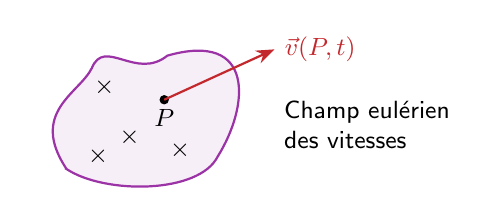
\begin{tikzpicture}[scale=.8]\blob\foreach\x/\y in{-.7/.5,-.3/-.3,.5/-.5,-.8/-.6}{\node at(\x,\y){$\times$};}\node[pt]at(.25,.3){};\node[below]at(.25,.3){$P$};\draw[cur](.25,.3)--(2,1.1)node[right]{$\vec v(P,t)$};\node[align=left,right]at(2,-.1){Champ eulérien\\des vitesses};\end{tikzpicture}}
\fig{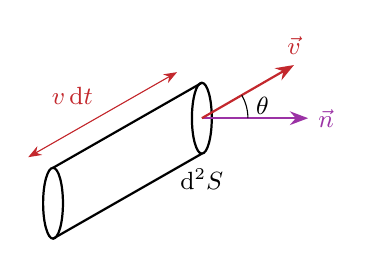
\begin{tikzpicture}[scale=.9]
\draw[thick](0,0)ellipse(.14 and .5);\draw[thick](2.1,1.2)ellipse(.14 and .5);\draw[thick](0,.5)--(2.1,1.7)(0,-.5)--(2.1,.7);
\draw[<->,current](-.35,.65)--(1.75,1.85)node[midway,above left]{$v\,\dd t$};
\draw[->,charge,thick](2.1,1.2)--(3.6,1.2)node[right]{$\vec n$};\draw[cur](2.1,1.2)--(3.4,1.95)node[above]{$\vec v$};\draw(2.75,1.2)arc(0:30:.65)node[midway,right]{$\theta$};\node[below]at(2.1,.63){$\dd^2S$};
\end{tikzpicture}}
$\dd^3q$ est la quantité de charge traversant $\dd^2S$ pendant $\dd t$.
% Source 15
\[\dd^3q=\rho(M,t)\bigl(\vec v(M,t)\cdot\dd^2\vec S\bigr)\dd t.\]
\begin{cadre}\[\vj(M,t)=\rho(M,t)\vec v(M,t).\]\end{cadre}
C'est le vecteur densité de courant de charges.
\begin{cadre}On définit le \textbf{vecteur densité de courant électrique} $\vj(M,t)$, dont le flux à travers une surface $\dd^2\vec S$ élémentaire est égal à la charge électrique qui traverse cette surface par unité de temps :
\[\vj(M,t)=\rho(M,t)\vec v(M,t).\]\end{cadre}
\Needspace{7\baselineskip}
Dans le cas général où il y a plusieurs types de porteurs de charges numérotés $i$, il faut ajouter les différents courants électriques associés aux différents porteurs de charges :
\begin{cadre}\[\vj(M,t)=\sum_i\rho_i(M,t)\vec v_i(M,t).\]\end{cadre}
\textbf{Remarque :} le vecteur densité de courant a pour unité $\mathrm{A\,m^{-2}}$.
\subsection{Intensité du courant traversant une surface}
% Sources 15-16

\[\dd q=\iint_\Sigma\vj(M,t)\cdot\dd^2\vec S\,\dd t.\]
\begin{cadre}\[I_\Sigma(t)=\iint_\Sigma\vj(M,t)\cdot\dd^2\vec S.\]\end{cadre}
$I_\Sigma(t)$ est l'intensité du courant à travers $\Sigma$.

Unité : $\mathrm A=\mathrm{C\,s^{-1}}$.
\subsection{Quelques ordres de grandeur pour le cuivre}
Pour un fil de cuivre utilisé en travaux pratiques :
\begin{itemize}\item Pour estimer la vitesse due à l'agitation thermique des porteurs de charge, on utilise le modèle de Drude : les électrons dans un conducteur sont comme des particules d'un gaz parfait.
\[\frac12m\langle v^2\rangle=\frac32k_BT,\qquad v_{\mathrm{th}}=\sqrt{\langle v^2\rangle}=\sqrt{\frac{3k_BT}{m}}\sim10^5\,\mathrm{m\,s^{-1}}.\]
\textbf{Remarque :} la vitesse moyenne de l'agitation thermique est nulle.
\item On prend l'exemple du cuivre : les porteurs de charges mobiles sont les électrons libres de masse $m=0{,}91\times10^{-30}\,\mathrm{kg}$ et de charge $e=-1{,}6\times10^{-19}\,\mathrm C$. Il y a environ un électron libre par atome.\end{itemize}
% Source 17
Connaissant la masse volumique du cuivre, $\mu=8{,}96\times10^3\,\mathrm{kg\,m^{-3}}$, et sa masse molaire, $M=63{,}5\,\mathrm{g\,mol^{-1}}$, on calcule la densité volumique des porteurs mobiles de charge $n$.
\titr{Modèle de Drude}
\fig{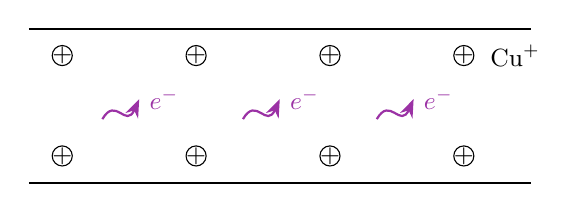
\begin{tikzpicture}[scale=.85]
\draw[thick](-.5,-.4)--(7,-.4)(-.5,1.9)--(7,1.9);
\foreach\x in{0,2,4,6}{\foreach\y in{0,1.5}{\draw(\x,\y)circle(.15);\node at(\x,\y){$+$};}}
\node[right]at(6.25,1.5){$\mathrm{Cu}^+$};
\foreach\x in{.6,2.7,4.7}{\draw[charge,->,thick](\x,.55)..controls(\x+.2,.9)and(\x+.35,.4)..(\x+.55,.85)node[right]{$e^-$};}
\end{tikzpicture}}
\Needspace{5\baselineskip}
Pour chaque atome, $\mathrm{Cu}$ donne :
\begin{itemize}\item un ion $\mathrm{Cu}^+$ sur le réseau cristallin fixe ;\item un électron $e^-$ qui contribue au courant.\end{itemize}
\[n(M,t)=\frac{\mu(M,t)}{M_{\mathrm{Cu}}}N_A.\]
\textbf{Application numérique :}
\[n=\frac{9\cdot10^3}{63\cdot10^{-3}}\bigl(6\cdot10^{23}\bigr)\simeq10^{29}\ \text{électrons}/\mathrm{m^3}.\]
% Source 18
\[|\rho|=n|q|=10^{29}\bigl(2\times10^{-19}\bigr)=2\times10^{10}\,\mathrm{C\,m^{-3}}.\]
\[I=jS,\qquad I\simeq1\,\mathrm A,\quad S\simeq1\,\mathrm{mm^2}.\]
\[j=\frac IS\simeq10^6\,\mathrm{A\,m^{-2}},\qquad v=\frac j{|\rho|}.\]

\[v=5\times10^{-5}\,\mathrm{m\,s^{-1}}=50\,\mathrm{\mu m\,s^{-1}}.\]
Cela représente quelques millimètres par minute : les électrons se déplacent extrêmement lentement. Cette vitesse est très petite devant la vitesse d'agitation thermique.
\subsection{Cas limite d'une distribution surfacique}
% Source 19
\fig{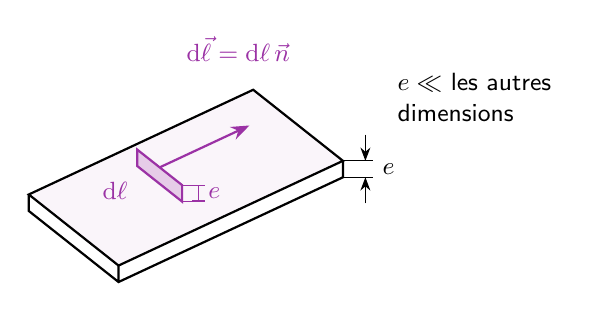
\begin{tikzpicture}[scale=.95]
\draw[thick,fill=charge!5](0,0)--(3,1.4)--(4.2,.45)--(1.2,-.95)--cycle;
\draw[thick](0,0)--(0,-.22)--(1.2,-1.17)--(4.2,.23)--(4.2,.45)(1.2,-1.17)--(1.2,-.95);
% Projection : section parallèle aux bords courts ; normale parallèle aux bords longs.
\filldraw[draw=charge,fill=charge!25,thick](1.45,.6)--(2.05,.125)--(2.05,-.095)--(1.45,.38)--cycle;
\node[charge,left]at(1.45,.05){$\dd\ell$};
\draw[charge,thin](2.05,.125)--(2.3,.125)(2.05,-.095)--(2.3,-.095);
\draw[charge,|-|](2.27,.125)--(2.27,-.095)node[midway,right]{$e$};
\draw[charge,->,thick](1.75,.3625)--(2.95,.9225);
\node[charge,above]at(2.8,1.65){$\dd\vec\ell=\dd\ell\,\vec n$};
\draw[thin](4.2,.23)--(4.6,.23)(4.2,.45)--(4.6,.45);
\draw[->](4.5,-.12)--(4.5,.23);\draw[->](4.5,.8)--(4.5,.45);\node[right]at(4.6,.34){$e$};
\node[align=left,right]at(4.8,1.3){$e\ll$ les autres\\dimensions};\end{tikzpicture}}
Le courant traversant $\dd\ell$ est :
\[\dd I=\vj(P,t)\cdot(\dd\ell\,e)\vec n=\vj(P,t)e\cdot\dd\ell\,\vec n,\qquad e\longrightarrow0.\]
On définit donc le vecteur densité de courant surfacique :
\[\vj_s(P,t)=\lim_{e\to0}\bigl(\vj(P,t)e\bigr).\]
\begin{cadre}\[\dd I=\vj_s(P,t)\cdot\dd\vec\ell.\]\end{cadre}
Unité : $\mathrm{A\,m^{-1}}$.
\begin{exemple}\textbf{Exemples :} un solénoïde, une nappe plane de courants.\end{exemple}
\subsection{Cas limite d'une distribution linéique}
% Sources 19-20
\fig{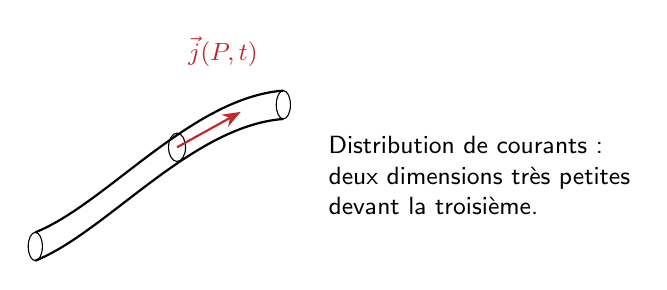
\begin{tikzpicture}[scale=.9]\draw[thick](0,-.2)..controls(1,.2)and(2.2,1.7)..(3.5,1.8);\draw[thick](0,.2)..controls(1,.6)and(2.2,2.1)..(3.5,2.2);\draw(0,0)ellipse(.1 and .2);\draw(3.5,2)ellipse(.1 and .2);\draw(2,1.4)ellipse(.12 and .2);\draw[cur](2,1.4)--(2.9,1.9);\node[current,above]at(2.65,2.4){$\vj(P,t)$};\node[align=left,right]at(4,1){Distribution de courants :\\deux dimensions très petites\\devant la troisième.};\end{tikzpicture}}
\[I=\lim_{S\to0}\bigl(j(P,t)S\bigr).\]
\fig{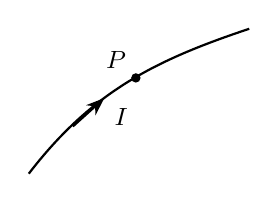
\begin{tikzpicture}[scale=.8]\draw[thick](-1.5,-.7)..controls(-.5,.6)and(.5,1.1)..(2,1.6);\draw[arr](-.8,.05)--(-.3,.5)node[below right]{$I$};\node[pt]at(.2,.82){};\node[above left]at(.2,.82){$P$};\end{tikzpicture}}
L'intensité du courant est :
\begin{cadre}\[I(P,t)=\frac{\dd q}{\dd t}.\]\end{cadre}
\begin{exemple}\textbf{Exemple : solénoïde.}
On utilise deux modèles : une distribution surfacique ou une distribution linéique.
\begin{center}
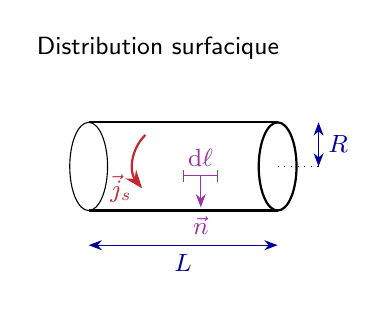
\begin{tikzpicture}[scale=.8]
\node[above]at(1.1,1.55){Distribution surfacique};
\draw[thick](0,-.7)--(3,-.7)(0,.7)--(3,.7);\draw(0,0)ellipse(.3 and .7);\draw[thick](3,0)ellipse(.3 and .7);
\draw[cur](.9,.5)..controls(.65,.25)and(.65,-.1)..(.85,-.35)node[left]{$\vj_s$};
\draw[charge,|-|](1.5,-.15)--(2.05,-.15)node[midway,above]{$\dd\ell$};\draw[charge,->](1.78,-.15)--(1.78,-.65)node[below]{$\vec n$};
\draw[<->,blue!60!black](3.65,0)--(3.65,.7)node[midway,right]{$R$};\draw[dotted](3,0)--(3.65,0);\draw[<->,blue!60!black](0,-1.25)--(3,-1.25)node[midway,below]{$L$};
\end{tikzpicture}\hspace{16mm}
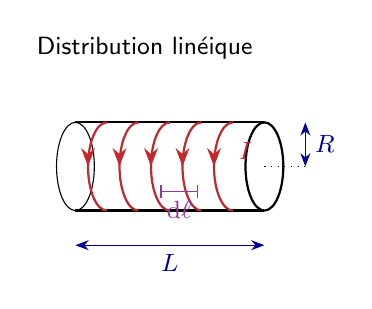
\begin{tikzpicture}[scale=.8]
\node[above]at(1.1,1.55){Distribution linéique};
\draw[thick](0,-.7)--(3,-.7)(0,.7)--(3,.7);\draw(0,0)ellipse(.3 and .7);\draw[thick](3,0)ellipse(.3 and .7);
\foreach\x in{.5,1,1.5,2,2.5}{\draw[current,thick,postaction={decorate},decoration={markings,mark=at position .5 with {\arrow{Stealth}}}](\x,.7)arc[start angle=90,end angle=270,x radius=.3,y radius=.7];}
\node[current]at(2.7,.25){$I$};\draw[charge,|-|](1.35,-.4)--(1.95,-.4)node[midway,below]{$\dd\ell$};
\draw[<->,blue!60!black](3.65,0)--(3.65,.7)node[midway,right]{$R$};\draw[dotted](3,0)--(3.65,0);\draw[<->,blue!60!black](0,-1.25)--(3,-1.25)node[midway,below]{$L$};\end{tikzpicture}
\end{center}
\[n_L=\frac{\text{nombre de spires}}{\text{longueur}}.\]
% Source 21
\fig{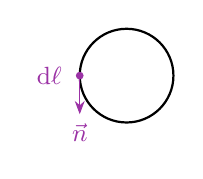
\begin{tikzpicture}[scale=.7]\draw[thick](0,0)circle(.85);\fill[charge](-.85,0)circle(2pt);\node[charge,left]at(-1,0){$\dd\ell$};\draw[charge,->](-.85,0)--(-.85,-.7)node[below]{$\vec n$};\end{tikzpicture}}
\[\dd I=j_s\dd\ell,\qquad\dd I=\underbrace{(n_L\dd\ell)}_{\text{nombre de spires dans }\dd\ell}I.\]
Donc :
\begin{cadre}\[j_s=n_LI.\]\end{cadre}
\end{exemple}
\subsection{Propriétés de symétrie}
\subsubsection{Symétrie plane}
\begin{cadre}[etoiles={\mathord{\star}\mkern5mu\mathord{\star}\mkern5mu\mathord{\star}\mkern5mu\mathord{\star}}]
\begin{minipage}{.49\linewidth}\centering\symfig{2}\end{minipage}\hfill
\begin{minipage}{.48\linewidth}Si $P\in\mathcal D$, alors
\[P'=\sym_\Pi(P)\in\mathcal D\]
et
\[\vj(P,t)=\sym_\Pi\bigl(\vj(P',t)\bigr).\]\end{minipage}
\end{cadre}
% Source 22
\begin{cadre}Une distribution de courants est \textbf{invariante par symétrie par rapport au plan $(\Pi)$} si, pour tout point $P$ de la distribution, son symétrique $P'$ par rapport au plan $(\Pi)$ appartient à la distribution et porte la densité volumique de courant symétrique de celle en $P$ :
\[\vj(P',t)=\sym_{(\Pi)}\bigl(\vj(P,t)\bigr).\]
$(\Pi)$ est un plan de symétrie de la distribution de courants.\end{cadre}
\begin{exemple}[unbreakable]\textbf{Exemples :}\fig{\solenoid{1}\hspace{20mm}\currentring{0}}\end{exemple}
\subsubsection{Antisymétrie plane}
\begin{cadre}[etoiles={\mathord{\star}\mkern5mu\mathord{\star}\mkern5mu\mathord{\star}\mkern5mu\mathord{\star}}]
\begin{minipage}{.49\linewidth}\centering\symfig{3}\end{minipage}\hfill
\begin{minipage}{.48\linewidth}Si $P\in\mathcal D$, alors
\[P'=\sym_\Pi(P)\in\mathcal D\]
et
\[\vj(P,t)=-\sym_\Pi\bigl(\vj(P',t)\bigr).\]\end{minipage}
\end{cadre}
% Source 23
\begin{cadre}Une distribution de courants \textbf{possède un plan d'antisymétrie $(\Pi)$} si, pour tout point $P$ de la distribution, son symétrique $P'$ par rapport au plan $(\Pi)$ appartient à la distribution et que les densités volumiques de courant en $P$ et $P'$ vérifient :
\[\vj(P',t)=-\sym_{(\Pi)}\bigl(\vj(P,t)\bigr).\]\end{cadre}
\begin{exemple}\textbf{Exemple :} une spire de courant circulaire.
\fig{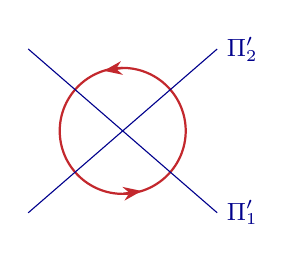
\begin{tikzpicture}[scale=.8]\draw[current,thick](0,0)circle(1);\draw[cur](0,-1)--(.3,-.954);\draw[cur](0,1)--(-.3,.954);\draw[plane](-1.5,-1.3)--(1.5,1.3)node[right]{$\Pi'_2$};\draw[plane](-1.5,1.3)--(1.5,-1.3)node[right]{$\Pi'_1$};\end{tikzpicture}}
\end{exemple}
\subsubsection{Invariance par translation}
\begin{cadre}Une distribution de courants est \textbf{invariante par translation parallèle à une direction $(D)$} si, pour tout point $P$ de la distribution, ses translatés parallèlement à $(D)$ appartiennent à la distribution et portent le même vecteur densité volumique de courants.\end{cadre}
% Source 24
\begin{exemple}\textbf{Exemples :}
\begin{itemize}\item Un solénoïde infini.\end{itemize}\fig{\solenoid{2}}
\begin{minipage}{\linewidth}\begin{itemize}\item Une nappe de courant plane infinie.\end{itemize}\fig{\sheet{1}}\end{minipage}\end{exemple}
\textbf{Remarque :} l'invariance par translation suppose une extension infinie de la distribution de courants. En pratique, cela signifie qu'une dimension de la distribution est très grande devant les autres longueurs de la distribution.
\subsubsection{Invariance par rotation}
\begin{cadre}Une distribution de courants est \textbf{invariante par rotation autour de l'axe $(\Delta)$} si, pour tout point $P$ de la distribution, ses transformés $P'$ par les rotations d'axe $(\Delta)$ d'angle $\alpha$ appartiennent à la distribution et si le vecteur densité volumique de courant $\vj(P',t)$ s'obtient à partir de $\vj(P,t)$ par rotation d'axe $(\Delta)$ et du même angle $\alpha$.
$(\Delta)$ est un axe de révolution ; la distribution possède la symétrie de révolution d'axe $(\Delta)$.\end{cadre}
% Source 25
\begin{exemple}\textbf{Exemples :}\fig{\currentring{1}\hspace{25mm}\solenoid{0}}\end{exemple}
\subsubsection{Distributions de haute symétrie}
Si la distribution de courants possède un grand nombre de propriétés de symétrie, elle est dite de haute symétrie et sa description se simplifie.
\begin{cadre}Une distribution de courants possède la \textbf{symétrie cylindrique} si elle est invariante par rotation autour d'un axe et par translation parallèlement à cet axe.\end{cadre}
\begin{cadre}Une distribution de courants possède la \textbf{symétrie sphérique} si elle est invariante par rotation autour de tout axe passant par un même point $O$. Le vecteur densité de courants ne dépend alors que de la distance à $O$ et est radial.\end{cadre}
% Source 26
\begin{exemple}\textbf{Solénoïde infini :}\fig{\solenoid{2}}
Il possède la symétrie cylindrique par rapport à $\Delta$.
\end{exemple}
\begin{exemple}\textbf{Courants à symétrie sphérique :} par exemple, dans un réacteur nucléaire, pour un noyau radioactif.
\fig{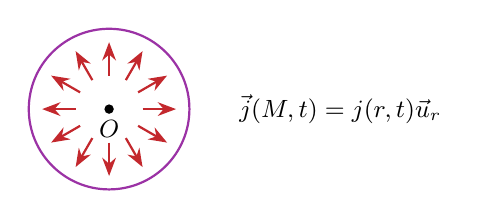
\begin{tikzpicture}[scale=.85]\draw[chg](0,0)circle(1.2);\node[pt]at(0,0){};\node[below]at(0,-.03){$O$};\foreach\a in{0,30,...,330}{\draw[cur](\a:.5)--(\a:1);}\node[right]at(1.8,0){$\vj(M,t)=j(r,t)\vec u_r$};\end{tikzpicture}}\end{exemple}
\section*{Tableau récapitulatif}
\renewcommand{\arraystretch}{1.7}
\begin{center}\begin{tabularx}{\linewidth}{|>{\centering\arraybackslash}X|>{\centering\arraybackslash}X|>{\centering\arraybackslash}X|}\hline
\textbf{Type de distribution}&\textbf{Charges}&\textbf{Courants}\\\hline
Volumique&$\rho(M,t)\quad(\mathrm{C\,m^{-3}})$&$\vj(M,t)\quad(\mathrm{A\,m^{-2}})$\\\hline
Surfacique&$\sigma(M,t)\quad(\mathrm{C\,m^{-2}})$&$\vj_s(M,t)\quad(\mathrm{A\,m^{-1}})$\\\hline
Linéique&$\lambda(M,t)\quad(\mathrm{C\,m^{-1}})$&$I(M,t)\quad(\mathrm A)$\\\hline
\end{tabularx}\end{center}
\end{document}